\chapter{System Design and Implementation} \label{ch:problem-solution}

This chapter describes the design and implementation of Pista in clear, practical terms. The goal is to provide consistent, accessible, and scalable pitch evaluations while keeping the system simple enough to maintain and study. The description focuses on what the system does today rather than speculative features.

\section{Solution Approach and Design Philosophy} \label{sec:solution-approach}

The solution targets three limits in startup evaluation: inconsistency, limited access, and scale. Standardized criteria reduce subjective variance. A web interface broadens access. Automated processing scales without fatigue effects. Pista uses GPT\,4 to produce structured, repeatable assessments across four dimensions with actionable feedback that helps founders and supports research.

\paragraph{Takeaway} The system applies a simple four-dimension rubric with a required Q\&A step to address inconsistency, access, and scale.

\section{System Architecture and Technical Implementation} \label{sec:system-design}

This section describes the current stack and the main data flows from input to evaluation and storage.

\subsection{Architecture Overview}\label{subsec:architecture-overview}
Pista is implemented as a three-tier web application. The presentation layer uses Next.js 15\footnote{\url{https://nextjs.org}} with React (App Router). The application layer exposes API routes for evaluation, transcription, and Q\&A. It also handles authentication. The data layer uses Convex\footnote{\url{https://www.convex.dev}} for real-time storage, reactive queries, and server functions. Clerk\footnote{\url{https://clerk.com}} provides authentication and organization contexts. The evaluation uses OpenAI GPT-4\footnote{\url{https://platform.openai.com}}. This stack replaced earlier experiments with NextAuth and PostgreSQL. The change simplified the system and improved iteration speed.

The overall workflow from user input to output is shown in Figure~\ref{fig:user-flow}. It shows the main steps and how data moves through the system.

\begin{figure}[H]
  \centering
  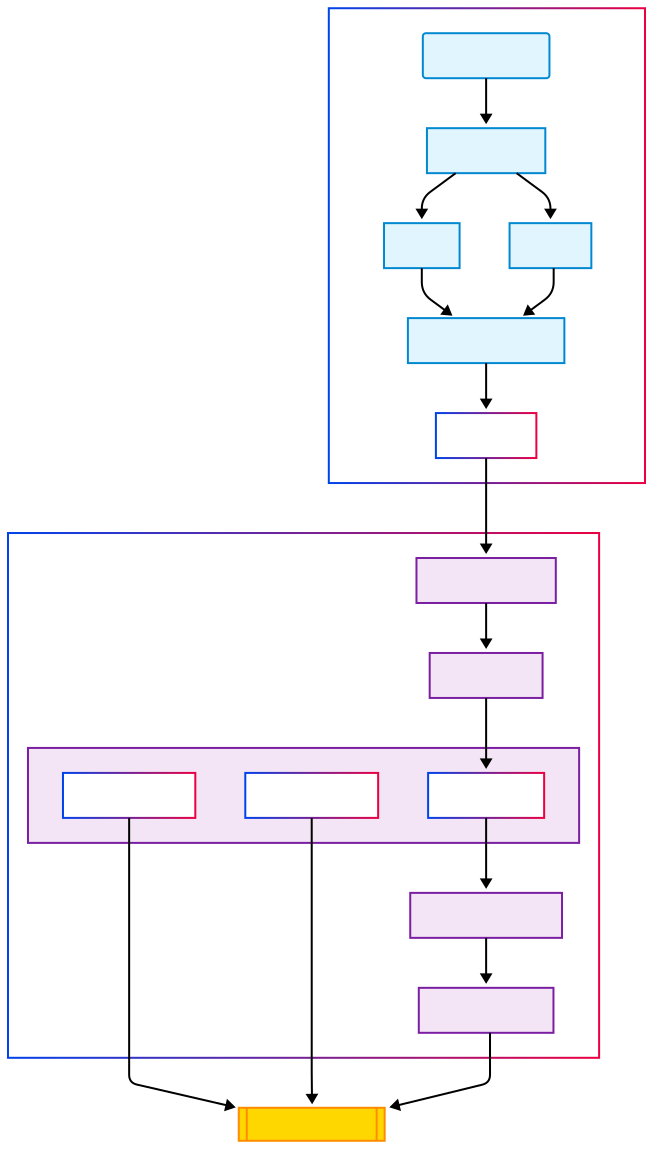
\includegraphics[width=0.85\textwidth]{img/user-diagram-flow}
\caption{High level workflow showing user interaction and data processing}
  \label{fig:user-flow}
\end{figure}

\subsection{Evaluation Framework}\label{subsec:evaluation-framework}
The evaluation framework combines standardized criteria with prompt engineering for consistent results. Four dimensions are used with fixed weights that match the implementation:

\begin{itemize}
  \item \textbf{Problem\mbox{-}Solution Fit} (0.30)
  \item \textbf{Business Model \& Market} (0.30)
  \item \textbf{Team \& Execution} (0.25)
  \item \textbf{Pitch Quality} (0.15)
\end{itemize}

Each dimension evaluates five aspects and yields a numeric score, plus strengths and improvements. Table~\ref{tab:criteria} summarizes the criteria and aspects used.

\begin{table}[H]
  \centering
  \caption{Evaluation criteria and aspects (summary)}
  \label{tab:criteria}
  \begin{tabular}{p{4cm} p{9cm}}
    \toprule
    \textbf{Criterion} & \textbf{Aspects} \\
    \midrule
    Problem\mbox{-}Solution Fit & Problem definition clarity; solution innovation; market understanding; competitive advantage; value proposition \\
    Business Model \& Market & Revenue model; market size \& growth; go-to-market strategy; customer acquisition; scalability potential \\
    Team \& Execution & Team capability; domain expertise; track record; resource management; implementation plan \\
    Pitch Quality & Clarity \& structure; data \& evidence; story \& engagement; Q\&A performance; overall persuasiveness \\
    \bottomrule
  \end{tabular}
\end{table}

The four dimensional processing flow is illustrated in Figure~\ref{fig:eval-flow}. This diagram matches the implemented single provider evaluation pipeline.

\paragraph{Takeaway} Fixed criteria and weights drive all evaluation results and enable reproducible comparisons.

\begin{figure}[H]
  \centering
  \includegraphics[width=0.9\textwidth]{img/eval-flow}
\caption{Evaluation and processing flow across four criteria}
  \label{fig:eval-flow}
\end{figure}

\subsection{AI Integration Strategy}\label{subsec:ai-integration-strategy}
The system uses GPT\,4 through OpenAI's API. Prompts return constrained JSON for reliable parsing. Ensemble or multi-provider evaluation is not part of the current implementation. It is left as future work if needed by the study design.

\paragraph{Prompt calibration} Initial evaluations showed a central tendency around 7/10. To improve spread and validity, we calibrated the scoring prompt. We added rubric anchors for the 1--10 scale. We added evidence gating that caps aspect scores at 4 when specifics are missing. We score aspects first and compute the criterion score as the rounded average. We also use a lower sampling temperature for scoring. The current configuration is tracked as \texttt{PROMPT\_VERSION = criteria\textrm{-}v1.2} and recorded in evaluation metadata.

\paragraph{Error handling} OpenAI calls use retries with exponential backoff for rate limits and transient failures. Responses are validated and mapped into strict application schemas before persistence.

\subsection{Data Models and Storage Architecture}\label{subsec:data-models-and-storage-architecture}
Convex stores pitches and user favorites with schema validation and indexed access. Each document is scoped by user and organization. Q\&A pairs are persisted with each pitch and reused when building evaluation input. Queries update the UI reactively without polling.

\paragraph{Schema overview} The \texttt{pitches} table stores the title, normalized text, type, and status. It also stores structured evaluation results, Q\&A pairs, organization id, user id, author name, and timestamps. Indexes include \texttt{by\_org}, \texttt{by\_user}, \texttt{by\_user\_org}, and \texttt{search\_title}. The \texttt{userFavorites} table links users and pitches with composite indexes.

\subsection{API Endpoints and Server Functions}\label{subsec:api-and-server}
\textbf{Next.js API routes}
\begin{itemize}
  \item \texttt{/api/evaluate} evaluates text using GPT\,4 (Edge runtime)
  \item \texttt{/api/generate-questions} produces up to three follow\mbox{-}up questions
  \item \texttt{/api/evaluate-answers} optional endpoint to update an evaluation using Q\&A responses (not used in the primary UI flow)
  \item \texttt{/api/transcribe} transcribes audio with Whisper\footnote{\url{https://openai.com/research/whisper}}
\end{itemize}

\textbf{Convex functions} (\texttt{convex/pitches.ts})
\begin{itemize}
  \item Mutations: \texttt{create}, \texttt{update}, \texttt{remove}, \texttt{favorite}, \texttt{unfavorite}, \texttt{prefetch}
  \item Queries: \texttt{get}, \texttt{getPitch}, \texttt{getFilteredPitches}, \texttt{getPitchStats}, \texttt{exportCSV}
\end{itemize}

\paragraph{Q\&A generation design} The question generator asks for 1--3 high priority, evidence seeking questions. It returns a structured JSON list tagged to an evaluation dimension. The route uses a lower sampling temperature for stability. If the model returns plain text, a numbered list fallback parser extracts up to three items. This improves evidence capture for the calibrated rubric without changing the original pitch content.

\paragraph{Takeaway} The primary path is transcribe (if audio) \textrightarrow{} generate questions \textrightarrow{} answer \textrightarrow{} evaluate \textrightarrow{} store.

\section{Authentication and Authorization Implementation}
Clerk handles sign in, session management, and organization contexts. Middleware protects routes and injects identity on the server. All Convex reads and writes are scoped by \texttt{userId} and \texttt{orgId}, which provides row level isolation without custom role tables.

\paragraph{Takeaway} Middleware protects app routes and row-level scoping enforces data isolation without complex roles.

\section{User Interface Implementation}
The frontend uses Next.js 15, React 18, and Tailwind CSS\footnote{\url{https://tailwindcss.com}}. Route groups organize the app into dashboard, pitch, and auth areas. Shared UI components live under \texttt{src/components/ui}; feature components live under \texttt{src/components/shared}. Lists support favorites, search, and filtering by score or date. The pitch view renders numeric scores and qualitative feedback with generated follow\mbox{-}up questions.

The pitch creation flow is shown in Figure~\ref{fig:user-flow-pitch}. It covers text input and audio uploads, Q\&A generation, evaluation, and Convex storage. In production use, the Q\&A step is required to capture missing evidence before scoring.

\begin{figure}[H]
  \centering
  \includegraphics[width=0.9\textwidth]{img/user-flow-pitch}
\caption{Pitch creation flow with Q\&A generation and Convex storage}
  \label{fig:user-flow-pitch}
\end{figure}

\paragraph{Takeaway} The UI guides users through a short, consistent flow and surfaces structured scores and feedback.

\section{Performance, Deployment, and Reliability}
\textbf{Performance} Virtualized lists keep lists responsive with large datasets. Code splitting defers non-critical UI. Reactive queries avoid manual polling.

\textbf{Deployment} API routes run on the Edge runtime where configured. Environment variables include the Convex URL, Clerk keys, and OpenAI API key. The same code paths run in development and production for result comparability.

\textbf{Reliability} API routes return clear error messages. The UI surfaces actionable feedback without exposing internal details.

\paragraph{Takeaway} Performance and deployment choices favor responsiveness and consistent behavior across environments.

\section{Implementation Results and User Experience}\label{sec:results}
Text-based evaluations typically complete within 30 to 60 seconds. Audio submissions require extra time for transcription. The interface is reactive, and list updates are visible without manual refresh. These results meet the design goals for responsive, consistent assessments suitable for research and iteration.

\paragraph{Scope} This chapter documents the implemented system. It does not cover earlier experiments with NextAuth and PostgreSQL, industry-specific weight profiles, or ensemble evaluation across multiple model providers. Those topics are left for future work and are referenced in the discussion as potential extensions.
% (Diagram source details moved to appendix for brevity.)
